\documentclass{article}

% --- load packages ---

\usepackage[margin=1in]{geometry} % change the margins
\usepackage{amsmath} % useful math environments and commands like align
\usepackage[colorlinks,bookmarks,bookmarksnumbered,allcolors=blue]{hyperref} % hyperlinks between references
\usepackage{graphicx}  % include images
\usepackage[caption=false]{subfig} % subfigures.  false option prevents conflicts in caption styling with other packages
\usepackage{booktabs} % better tables
\usepackage[capitalise]{cleveref} % better referencing. uses cref.
\usepackage[section]{placeins} % sometimes useful to prevent figures from floating out of a section
\usepackage{cite} % handles multiple citations in one command better
\usepackage{doi} % allow correct hypderlinking of DOIs
\usepackage{hyperref}


\begin{document}

\title{Homework 3}
\author{Jaron Ellingson}
% put in \date{} if you don't want a date to appear, or enter a specific date, otherwise default is today's date.
\maketitle

 %\href{https://byu.box.com/shared/static/anxheci3eytucrh3ke57k2sqdx0ivmjg.pdf}{homework pdf}

\section*{Computing Derivatives}

The following describes and compares several methods for computing derivatives for constrained optimization problems. I choose to implement these methods to solve the 10 member truss problem which seeks to minimize the mass of a 10-truss structure that holds a load suspended horizontally from a wall  while also holding the loads placed on the structure (\cref{fig:truss}). This problem 

\begin{equation*}
\begin{aligned}
\text{minimizes} & \quad J= \sum_{i=1}^{n} Mass(A_i) \\
\text{with respect to} & \quad A_1 ... A_{n} \\
\text{subject to} & \quad A_i \ge 0.1 \quad \text{and} \quad | \sigma_i | \le \sigma_y \quad \forall i=1 ... n,
\end{aligned}
\end{equation*}

where $A_i$ is the cross-sectional area, $\sigma_i$ is the corresponding stress, and $\sigma_y$ is the yield stress. Please see this see \href{https://byu.box.com/shared/static/h8gzy7nuzzk42ta7388y1luj3yhgsltq.pdf}{handout} for further details.


\begin{figure}[htbp]
	\centering
	
	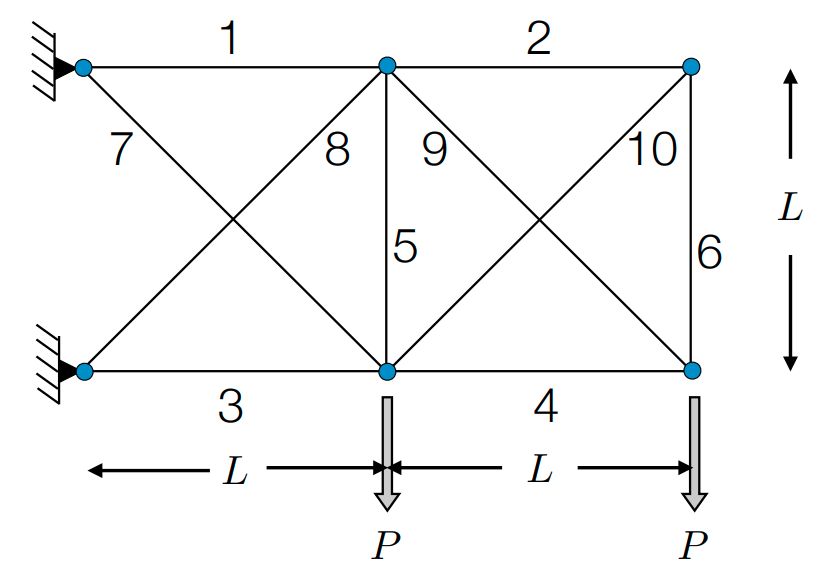
\includegraphics[width=0.75\textwidth]{truss.png}
	
	\caption{Truss}
	\label{fig:truss}
\end{figure}

To effectively solve this problem, the optimization methods requires derivatives to be computed. More precisely we need the function  and constraint derivatives or 


\begin{equation}
\frac{\partial m}{\partial A}=
\begin{bmatrix} 
\frac{\partial m}{\partial A_1} \\
\vdots \\
\frac{\partial m}{\partial A_{n_x}}
\end{bmatrix}
\end{equation}

and 

\begin{equation}
\frac{\partial \sigma}{\partial A}=
\begin{bmatrix} 
\frac{\partial \sigma_1}{\partial A_1} & \dots & \frac{\partial \sigma_i}{\partial A_{n_x}} \\
\vdots & \ddots & \\
\frac{\partial \sigma_{n_f}}{\partial A_1} &        & \frac{\partial \sigma_{n_f}}{\partial A_{n_x}} 
\end{bmatrix},
\end{equation}

where m is the mass of the truss, $n_x$ is the number of truss areas, and $n_f$ is the number of constrained stress elements. In this problem $n_x=n_f$. For a more complete derivation of each of the methods, please consult the \href{https://byu.box.com/shared/static/17bqmaop0v1o0fwqg1etx7dofl6ad35t.pdf}{textbook}.

\subsection*{Finite Difference}

The first group of methods are called the finite-difference approximations. These methods are all derived by combining Taylor series expansions,

$$ f(x+h\hat{e}_j)=f(x)+h\frac{\partial f}{\partial x_j} + \frac{h^2}{2!}\frac{\partial^2f}{\partial x_j^2}+\frac{h^3}{3!}\frac{\partial^3f}{\partial x_j^3
} + \dots $$

where $h$ is a step size and $\hat{e}_j$ is the unit vector in the $j^{th}$ direction. I choose to implement the central difference method, which combines both the forward and the backward finite difference to obtain a more accurate approximation of the derivatives. The final equation is 

$$ \frac{\partial f}{\partial x_i} = \frac{f(x+h\hat{e}_j) - f(x-h\hat{e}_j)}{2h} + O(h^2), $$

where the $O(h^2)$ represents higher squared terms omitted from the Taylor series expansions. 

The limitation of this method is that you have to evaluate the function for every design variable twice. This means that for the truss problem we need to evaluate the function 10x2=20 times for each gradient approximation. Additionally, this method has truncation and subtraction cancellation errors. The advantage of this method is that it can operate with black boxes, i.e. you don't need access to source code.

\subsection*{Complex Step}

The complex step is similar to the finite-difference step but requires access to the sources code to ensure that the complex values are appropriately calculated. We once again formulate the Taylor series but we take a step in the complex direction, 

$$ f(x+ih\hat{e}_j)=f(x)+ih\frac{\partial f}{\partial x_j} - \frac{h^2}{2!}\frac{\partial^2f}{\partial x_j^2}-i\frac{h^3}{3!}\frac{\partial^3f}{\partial x_j^3
} + \dots .$$

We then take the imaginary part of both sides and rearrange to get

$$ \frac{\partial f}{\partial x_i} = \frac{Im[f(x+ih\hat{e}_j)]}{h} + O(h^3). $$

This method allows for greater precision, almost exact derivatives up to the function precision.

\subsection*{Algorithmic Differentiation}

The algorithmic differentiation (AD) method is based on the differentiation chain rule. This means that you can build the derivative as you apply the objective function. The AD method has a forward mode and a reverse mode. We choose to implement the forward mode which can be written as:

$$ \frac{dv_i}{dv_j}=\sum_{k=j}^{i-1}\frac{\partial V_i}{\partial v_k}\frac{dv_k}{dv_j}.$$ 

We choose to implement this method using a python library called \href{https://pythonhosted.org/algopy/}{AlgoPy}. The AD method can have precision matching the function evaluation but needs access to the source code.

\subsection*{Adjoint}

The final method is called the Adjoint method, or analytic method. This method linearizes the model to obtain a system of linear equations. The derivative is then calculated by solving for the unknown variables. The method first creates a sets of residuals that need to be driven to zero, $ r = R(x,y(x)) = 0,$ and functions of interest, $ f=F(x,y(x)). $ We then can apply the chain rule to fine the total derivative of f to get,

$$ \frac{df}{dx}=\frac{\partial F}{\partial x}-\frac{\partial F}{\partial y}\left[\frac{\partial R}{\partial y}\right]^{-1} \frac{\partial R}{\partial x}.$$

In our case we need to find the derivative of stress with respect to area. We choose our residual to be $R=Kd-F$, where $K$ is a stiffness matrix, $d$ is a displacement vector, and $F$ is our forces. Our output equation or function of interest is $\sigma=Sd$, with $S$ being a stress matrix. Therefore, our derivative equation becomes,

$$ \frac{d\sigma}{dA}=\frac{\partial \sigma}{\partial A}-\frac{\partial \sigma}{\partial d}\left[\frac{\partial R}{\partial d}\right]^{-1} \frac{\partial R}{\partial A}.$$

The adjoint method is considered the most accurate of the methods because it is analytical. This method also needs access to the source code.

\section*{Average Relative Errors}

I will now compare the relative errors of each of the methods when compared to the Adjoint method. \Cref{tab:comp_der} shows the average relative errors for 100 uniform random areas points spread from 0.1 to 20 $m^2$. For the mass derivative, the complex step and algorithmic differentiation were analytically accurate while the finite-difference was accurate up to 5.3e-5. The stress derivative is the same as result but slightly less accurate for all three methods. 

\begin{table}[htb]
	\centering
	\caption{Average relative error for each method with 100 uniformly random starting points.}
	\label{tab:comp_der}
	\begin{tabular}{c|c|c}
		\toprule
		Algorithm & Mass Derivative & Stress Derivative \\
		\midrule
		Finite-Difference & 5.347291203789755e-05 & 0.02727215090088324 \\
		Complex-Step  & 0.0 & 3.336212472827231e-10 \\
		Algorithmic Differentiation & 0.0 & 2.1207032039874913e-11 \\
		\bottomrule
	\end{tabular}
\end{table}

\section*{Convergence}

I next performed the actual optimization for the truss problem using the python library \href{https://docs.scipy.org/doc/scipy/reference/generated/scipy.optimize.minimize.html}{scipy} for the finite-difference method and the adjoint method. \Cref{tab:c} shows the average number of function evaluations and time to solve for each method. I used 25 uniformly random starting areas ranging from 0.1 to 20 $m^2$.
\Cref{fig:opt10} shows the corresponding convergence plots for each of the methods. Notice that the finite-difference method took roughly 10x or more function calls to converge and appears to be more likely to diverge in the middle than the adjoint method. This is because the finite-difference methods depend on evaluating the function proportional to the number of the design variables and is less accurate than the analytical derivative that the adjoint method provides. 

\begin{table}[htb]
	\centering
	\caption{Average function evaluations and time to solve for the finite-difference and adjoint methods for 25 uniformly random starting points.}
	\label{tab:c}
	\begin{tabular}{c|c|c}
		\toprule
		Algorithm & Function Evaluations & Time to Solve (sec) \\
		\midrule
		Finite-Difference & 386.0 & 3.3085175704956056\\
		Adjoint & 32.96 & 0.25411544799804686 \\
		\bottomrule
	\end{tabular}
\end{table}

\begin{figure}[htbp]
	\centering

	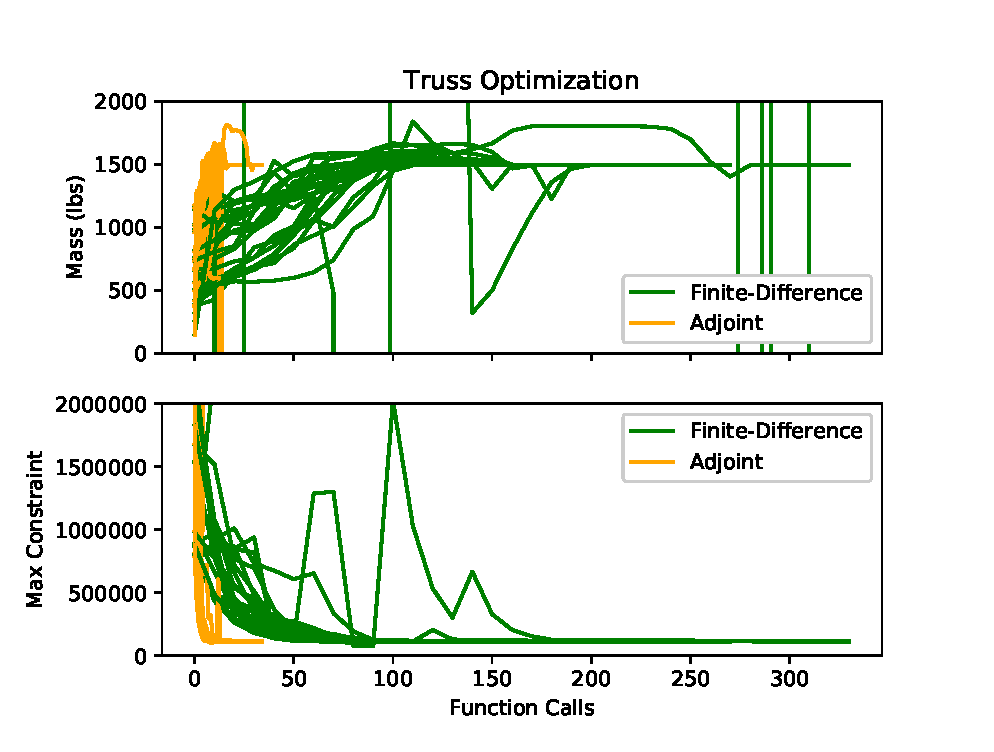
\includegraphics[width=0.75\textwidth]{optimality10.eps}

	\caption{Convergence plots of mass and max constraint values fro each function call. The starting points were 25 uniformly random starting areas ranging from 0.1 to 20 $m^2$.}
	\label{fig:opt10}
\end{figure}

\section*{Discussion}

Overall it is really efficient for me to calculate the derivatives for a optimization scheme because it means less function calls and reduces the time to solve by an order of 10. The three most accurate methods, complex-step, algorithmic differentiation, and adjoint, each require knowledge of the source code and increase in complexity. If I were to pick, the algorithmic differentiation seems to be the best if you cannot formulate the adjoint method because there are libraries that can help you build the differentiation chain. The adjoint method is the best choice overall because we were able to formulate the residual and solve accordingly. The finite-difference methods are great for black box optimization. 

% This is for the bibliography.  Note that it is using sample.bib 
% you would need to provide your own bibtex file.

%\bibliographystyle{unsrt}
%\bibliography{sample}




\end{document}